

%% 12. Modeling by Example

% AXPY on GPUs and MIC in offload mode

% \begin{frame}{Performance Modeling: Vector Addition}
% 
%  \begin{block}{Vector Addition}
%   \begin{itemize}
%    \item $x = y + z$ with $N$ elements each
%    \item 1 FLOP per 24 byte in double precision
%    \item Limited by memory bandwidth $\Rightarrow T_1(N) \stackrel{?}{\approx} 3 \times 8 \times N / \mathrm{Bandwidth}$
%   \end{itemize}
%  \end{block}
% 
%  \vspace*{-0.5cm}
%  \begin{center}
%   \only<1>{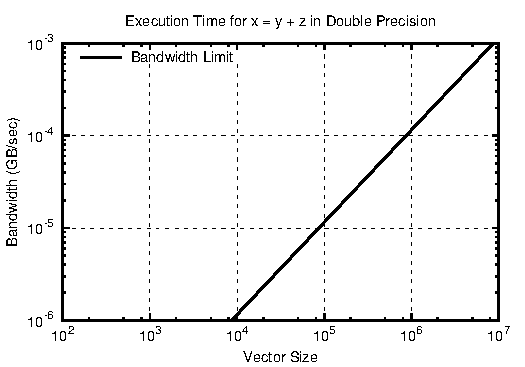
\includegraphics[width=0.75\textwidth]{figures/vector-addition-time-0}}
%   
%   \only<2>{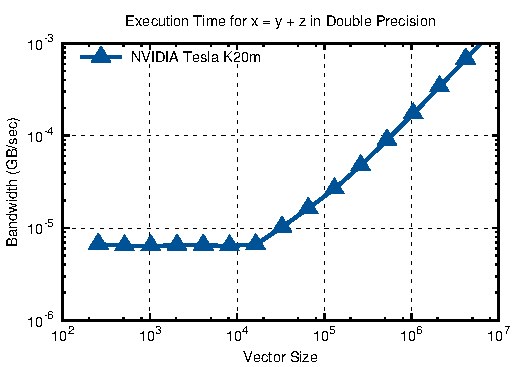
\includegraphics[width=0.75\textwidth]{figures/vector-addition-time-1}}
%   
%   \only<3>{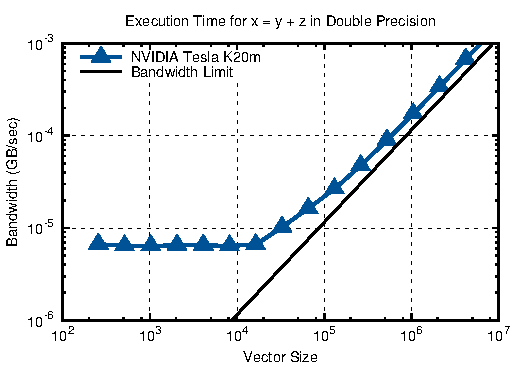
\includegraphics[width=0.75\textwidth]{figures/vector-addition-time-2}}
%   
%  \end{center}
% 
% \end{frame}


\begin{frame}{Performance Modeling: Vector Addition}

 \begin{block}{Vector Addition}
  \begin{itemize}
   \item $x = y + z$ with $N$ elements each
   \item 1 FLOP per 24 byte in double precision
   \item Limited by memory bandwidth $\Rightarrow T_2(N) \stackrel{?}{\approx} 3 \times 8 \times N / \mathrm{Bandwidth} + \mathrm{Latency}$
  \end{itemize}
 \end{block}

 \vspace*{-0.5cm}
 \begin{center}
  \only<1>{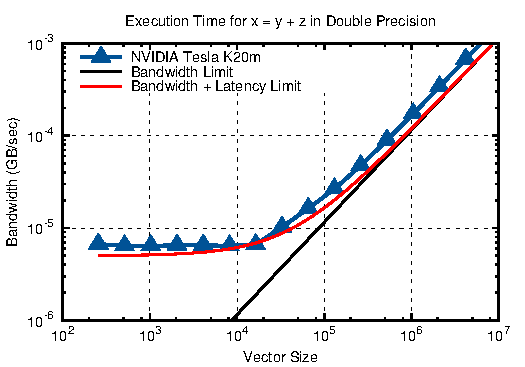
\includegraphics[width=0.75\textwidth]{figures/vector-addition-time-3}}
  
  \only<2>{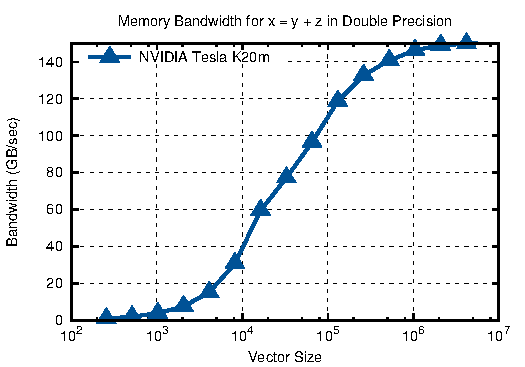
\includegraphics[width=0.75\textwidth]{figures/vector-addition-bw}}
 \end{center}
 
 \end{frame}

 
%%%%%%%%%%%

\begin{frame}{Performance Modeling: Matrix-Matrix Products}


 \begin{center}
  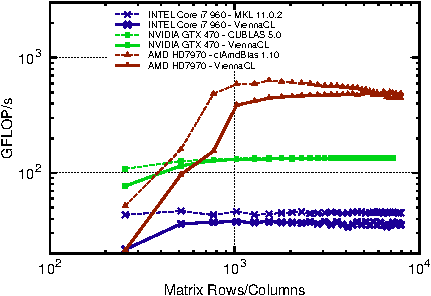
\includegraphics[width=0.95\textwidth]{figures/dgemm}
 \end{center}
 
 \end{frame}

%%
%% Conjugate Gradients: Pipelining
%%

% Show CG algorithm <-> BLAS
% \begin{frame}[fragile]{Performance Modeling: Conjugate Gradients}
% 
%  \begin{block}{}
%   
%    \begin{minipage}{0.45\textwidth}
%       {\large \textbf{Pseudocode}} \\
%       
%       Choose $x_0$ \\
%       $p_0 = r_0 = b - Ax_0$ \\
%       For $i=0$ until convergence
%      \begin{enumerate}
%       \item Compute and store $Ap_i$
%       \item Compute $\langle p_i, Ap_i \rangle$
%       \item $\alpha_i = \langle r_i, r_i \rangle / \langle p_i, Ap_i \rangle$
%       \item $x_{i+1} = x_{i} + \alpha_i p_i$          
%       \item $r_{i+1} = r_i - \alpha_i Ap_i$       
%       \item Compute $\langle r_{i+1}, r_{i+1} \rangle$
%       \item $\beta_i = \langle r_{i+1}, r_{i+1} \rangle / \langle r_i, r_i \rangle$
%       \item $p_{i+1} = r_{i+1} + \beta_i p_i$
%      \end{enumerate}
%      EndFor
%    \end{minipage}
%    \begin{minipage}{0.48\textwidth}
%       {\large \textbf{BLAS-based Implementation}} \\
%       
%             - \\
%       SpMV, AXPY \\
%       For $i=0$ until convergence
%      \begin{enumerate}
%       \item SpMV
%       \item DOT
%       \item -
%       \item AXPY         
%       \item AXPY
%       \item DOT
%       \item -
%       \item AXPY
%      \end{enumerate}
%      EndFor
%    \end{minipage}
%    
%    \end{block}
%    
% \end{frame}
% 
% 
% \begin{frame}[fragile]{Performance Modeling: Conjugate Gradients}
% 
%  \begin{block}{}
%   
%    \begin{minipage}{0.45\textwidth}
%       {\large \textbf{Pseudocode}} \\
%       
%       Choose $x_0$ \\
%       $p_0 = r_0 = b - Ax_0$ \\
%       For $i=0$ until convergence
%      \begin{enumerate}
%       \item Compute and store $Ap_i$
%       \item Compute $\langle p_i, Ap_i \rangle$
%       \item $\alpha_i = \langle r_i, r_i \rangle / \langle p_i, Ap_i \rangle$
%       \item $x_{i+1} = x_{i} + \alpha_i p_i$          
%       \item $r_{i+1} = r_i - \alpha_i Ap_i$       
%       \item Compute $\langle r_{i+1}, r_{i+1} \rangle$
%       \item $\beta_i = \langle r_{i+1}, r_{i+1} \rangle / \langle r_i, r_i \rangle$
%       \item $p_{i+1} = r_{i+1} + \beta_i p_i$
%      \end{enumerate}
%      EndFor
%    \end{minipage}
%    \begin{minipage}{0.48\textwidth}
%       {\large \textbf{BLAS-based Implementation}} \\
%       
%             - \\
%       SpMV, AXPY \\
%       For $i=0$ until convergence
%      \begin{enumerate}
%       \item SpMV
%       \item DOT {\color{red} $\leftarrow$ Global sync!}
%       \item -
%       \item AXPY         
%       \item AXPY
%       \item DOT {\color{red} $\leftarrow$ Global sync!}
%       \item -
%       \item AXPY
%      \end{enumerate}
%      EndFor
%    \end{minipage}
%    
%    \end{block}
%    
% \end{frame}


\begin{frame}[fragile]{Performance Modeling: Conjugate Gradients}

 \begin{block}{}
  
   \begin{minipage}{0.45\textwidth}
      {\large \textbf{Pseudocode}} \\
      
      Choose $x_0$ \\
      $p_0 = r_0 = b - Ax_0$ \\
      For $i=0$ until convergence
     \begin{enumerate}
      \item Compute and store $Ap_i$
      \item Compute $\langle p_i, Ap_i \rangle$
      \item $\alpha_i = \langle r_i, r_i \rangle / \langle p_i, Ap_i \rangle$
      \item $x_{i+1} = x_{i} + \alpha_i p_i$          
      \item $r_{i+1} = r_i - \alpha_i Ap_i$       
      \item Compute $\langle r_{i+1}, r_{i+1} \rangle$
      \item $\beta_i = \langle r_{i+1}, r_{i+1} \rangle / \langle r_i, r_i \rangle$
      \item $p_{i+1} = r_{i+1} + \beta_i p_i$
     \end{enumerate}
     EndFor
   \end{minipage}
   \begin{minipage}{0.48\textwidth}
      {\large \textbf{BLAS-based Implementation}} \\
      
            - \\
      SpMV, AXPY \\
      For $i=0$ until convergence
     \begin{enumerate}
      \item SpMV {\color{blue} $\leftarrow$ No caching of $Ap_i$}
      \item DOT {\color{red} $\leftarrow$ Global sync!}
      \item -
      \item AXPY         
      \item AXPY  {\color{blue} $\leftarrow$ No caching of $r_{i+1}$}
      \item DOT {\color{red} $\leftarrow$ Global sync!}
      \item -
      \item AXPY
     \end{enumerate}
     EndFor
   \end{minipage}
   
   \end{block}
   
\end{frame}

\begin{frame}[fragile]{Performance Modeling: Conjugate Gradients}

 \begin{block}{}
 
 \begin{center}
  \vspace*{-0.5cm}
  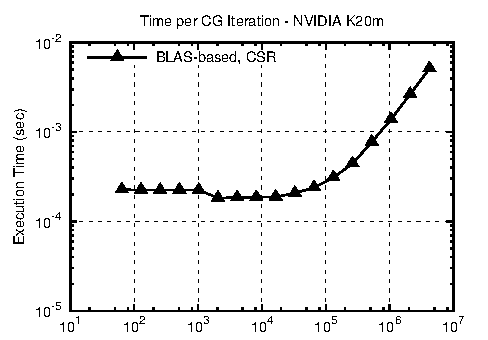
\includegraphics[width=0.85\textwidth]{figures/cg-k20m-0}
 \end{center}

 \begin{itemize}
  \item   \vspace*{-0.3cm} {\small (2D Finite Difference Discretization)}
 \end{itemize}

 \end{block}
   
\end{frame}


\begin{frame}[fragile]{Performance Modeling: Conjugate Gradients}

 \begin{block}{Performance Modeling}
   \begin{itemize}
    \item 6 Kernel Launches (plus two for reductions)
    \item Two device to host data reads from dot products
    \item Model SpMV as seven vector accesses (5-point stencil)
    \item $T(N) = 8 \times 10^{-6} + 2 \times 2 \times 10^{-6} + (7+2+3+3+2+3) \times 8 \times x / \mathrm{Bandwidth}$
   \end{itemize}

 
 \begin{center}
  \vspace*{-0.2cm}
  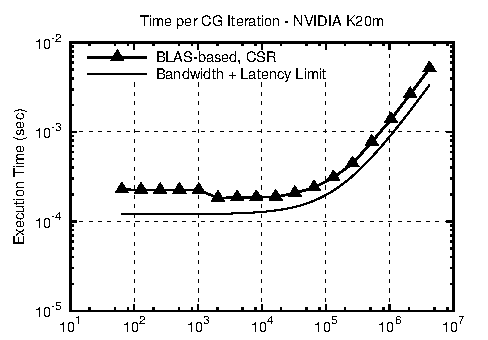
\includegraphics[width=0.65\textwidth]{figures/cg-k20m-1}
 \end{center}

 \begin{itemize}
  \item   \vspace*{-0.5cm} {\small (2D Finite Difference Discretization)}
 \end{itemize}

 \end{block}
   
\end{frame}


%%%%%%%%

% Step 3: Show and discuss pipelined/improved version

\begin{frame}[fragile]{Performance Modeling: Conjugate Gradient Optimizations}

 \begin{block}{Optimization: Rearrange the algorithm}
   \begin{itemize}
   \item  Remove unnecessary reads 
   \item  Remove unnecessary synchronizations
   \item Use custom kernels instead of standard BLAS
  \end{itemize}
 \end{block}
   
\end{frame}


% \begin{frame}[fragile]{Performance Modeling: Conjugate Gradients}
% 
%  \begin{block}{}
%   
%    \begin{minipage}{0.45\textwidth}
%       {\large \textbf{Standard CG}} \\
%       
%       Choose $x_0$ \\
%       $p_0 = r_0 = b - Ax_0$ \\
%       For $i=0$ until convergence
%      \begin{enumerate}
%       \item Compute and store $Ap_i$
%       \item Compute $\langle p_i, Ap_i \rangle$
%       \item $\alpha_i = \langle r_i, r_i \rangle / \langle p_i, Ap_i \rangle$
%       \item $x_{i+1} = x_{i} + \alpha_i p_i$          
%       \item $r_{i+1} = r_i - \alpha_i Ap_i$       
%       \item Compute $\langle r_{i+1}, r_{i+1} \rangle$
%       \item $\beta_i = \langle r_{i+1}, r_{i+1} \rangle / \langle r_i, r_i \rangle$
%       \item $p_{i+1} = r_{i+1} + \beta_i p_i$
%      \end{enumerate}
%      EndFor
%    \end{minipage}
%    \begin{minipage}{0.53\textwidth}
%    \end{minipage}
%    
%    \end{block}
%    
% \end{frame}

% 
% \begin{frame}[fragile]{Performance Modeling: Conjugate Gradients}
% 
%  \begin{block}{}
%   
%    \begin{minipage}{0.45\textwidth}
%       {\large \textbf{Standard CG}} \\
%       
%       Choose $x_0$ \\
%       $p_0 = r_0 = b - Ax_0$ \\
%       For $i=0$ until convergence
%      \begin{enumerate}
%       \item Compute and store $Ap_i$
%       \item Compute $\langle p_i, Ap_i \rangle$
%       \item $\alpha_i = \langle r_i, r_i \rangle / \langle p_i, Ap_i \rangle$
%       \item $x_{i+1} = x_{i} + \alpha_i p_i$          
%       \item $r_{i+1} = r_i - \alpha_i Ap_i$       
%       \item Compute $\langle r_{i+1}, r_{i+1} \rangle$
%       \item $\beta_i = \langle r_{i+1}, r_{i+1} \rangle / \langle r_i, r_i \rangle$
%       \item $p_{i+1} = r_{i+1} + \beta_i p_i$
%      \end{enumerate}
%      EndFor
%    \end{minipage}
%    \begin{minipage}{0.53\textwidth}
%       {\large \textbf{Pipelined CG}} \\
%       
%       Choose $x_0$ \\
%       $p_0 = r_0 = b - Ax_0$ \\
%       For $i=1$ until convergence
%      \begin{enumerate}
%       \item $i=1$: Compute $\alpha_0$, $\beta_0$, $Ap_0$
%       \item $x_i = x_{i-1} + \alpha_{i-1} p_{i-1}$          
%       \item $r_i = r_{i-1} - \alpha_{i-1} Ap_i$       
%       \item $p_i = r_i + \beta_{i-1} p_{i-1}$       
%       \item Compute and store $Ap_i$
%       \item Compute $\langle Ap_i, Ap_i \rangle$, $\langle p_i, Ap_i \rangle$, $\langle r_i, r_i \rangle$
%       \item $\alpha_i = \langle r_i, r_i \rangle / \langle p_i, Ap_i \rangle$
%       \item $\beta_i = ( \alpha_i^2 \langle Ap_i, Ap_i \rangle - \langle r_i, r_i \rangle) / \langle r_i, r_i \rangle$
%      \end{enumerate}
%      EndFor
%    \end{minipage}
%    
%    \end{block}
%    
% \end{frame}
% 
% \begin{frame}[fragile]{Performance Modeling: Conjugate Gradients}
% 
%  \begin{block}{}
%   
%    \begin{minipage}{0.45\textwidth}
%       {\large \textbf{Standard CG}} \\
%       
%       Choose $x_0$ \\
%       $p_0 = r_0 = b - Ax_0$ \\
%       For $i=0$ until convergence
%      \begin{enumerate}
%       \item Compute and store $Ap_i$
%       \item Compute $\langle p_i, Ap_i \rangle$
%       \item $\alpha_i = \langle r_i, r_i \rangle / \langle p_i, Ap_i \rangle$
%       \item $x_{i+1} = x_{i} + \alpha_i p_i$          
%       \item $r_{i+1} = r_i - \alpha_i Ap_i$       
%       \item Compute $\langle r_{i+1}, r_{i+1} \rangle$
%       \item $\beta_i = \langle r_{i+1}, r_{i+1} \rangle / \langle r_i, r_i \rangle$
%       \item $p_{i+1} = r_{i+1} + \beta_i p_i$
%      \end{enumerate}
%      EndFor
%    \end{minipage}
%    \begin{minipage}{0.53\textwidth}
%       {\large \textbf{Pipelined CG}} \\
%       
%       Choose $x_0$ \\
%       $p_0 = r_0 = b - Ax_0$ \\
%       For $i=1$ until convergence
%      \begin{enumerate}
%       \item $i=1$: Compute $\alpha_0$, $\beta_0$, $Ap_0$
%       \item {\color{blue}$x_i = x_{i-1} + \alpha_{i-1} p_{i-1}$}
%       \item {\color{blue}$r_i = r_{i-1} - \alpha_{i-1} Ap_i$}
%       \item {\color{blue}$p_i = r_i + \beta_{i-1} p_{i-1}$}       
%       \item Compute and store $Ap_i$
%       \item Compute $\langle Ap_i, Ap_i \rangle$, $\langle p_i, Ap_i \rangle$, {\color{blue}$\langle r_i, r_i \rangle$}
%       \item $\alpha_i = \langle r_i, r_i \rangle / \langle p_i, Ap_i \rangle$
%       \item $\beta_i = ( \alpha_i^2 \langle Ap_i, Ap_i \rangle - \langle r_i, r_i \rangle) / \langle r_i, r_i \rangle$
%      \end{enumerate}
%      EndFor
%    \end{minipage}
%    
%    \end{block}
%    
% \end{frame}


\begin{frame}[fragile]{Performance Modeling: Conjugate Gradients}

 \begin{block}{}
  
   \begin{minipage}{0.45\textwidth}
      {\large \textbf{Standard CG}} \\
      
      Choose $x_0$ \\
      $p_0 = r_0 = b - Ax_0$ \\
      For $i=0$ until convergence
     \begin{enumerate}
      \item Compute and store $Ap_i$
      \item Compute $\langle p_i, Ap_i \rangle$
      \item $\alpha_i = \langle r_i, r_i \rangle / \langle p_i, Ap_i \rangle$
      \item $x_{i+1} = x_{i} + \alpha_i p_i$          
      \item $r_{i+1} = r_i - \alpha_i Ap_i$       
      \item Compute $\langle r_{i+1}, r_{i+1} \rangle$
      \item $\beta_i = \langle r_{i+1}, r_{i+1} \rangle / \langle r_i, r_i \rangle$
      \item $p_{i+1} = r_{i+1} + \beta_i p_i$
     \end{enumerate}
     EndFor
   \end{minipage}
   \begin{minipage}{0.53\textwidth}
      {\large \textbf{Pipelined CG}} \\
      
      Choose $x_0$ \\
      $p_0 = r_0 = b - Ax_0$ \\
      For $i=1$ until convergence
     \begin{enumerate}
      \item $i=1$: Compute $\alpha_0$, $\beta_0$, $Ap_0$
      \item {\color{blue}$x_i = x_{i-1} + \alpha_{i-1} p_{i-1}$}
      \item {\color{blue}$r_i = r_{i-1} - \alpha_{i-1} Ap_i$}
      \item {\color{blue}$p_i = r_i + \beta_{i-1} p_{i-1}$}       
      \item {\color{red} Compute and store $Ap_i$}
      \item  {\color{red} Compute $\langle Ap_i, Ap_i \rangle$, $\langle p_i, Ap_i \rangle$}, {\color{blue}$\langle r_i, r_i \rangle$}
      \item $\alpha_i = \langle r_i, r_i \rangle / \langle p_i, Ap_i \rangle$
      \item $\beta_i = ( \alpha_i^2 \langle Ap_i, Ap_i \rangle - \langle r_i, r_i \rangle) / \langle r_i, r_i \rangle$
     \end{enumerate}
     EndFor
   \end{minipage}
   
   \end{block}
   
\end{frame}


\begin{frame}[fragile]{Performance Modeling: Conjugate Gradients}
 \begin{block}{}
 \begin{center}
  \vspace*{-0.5cm}
  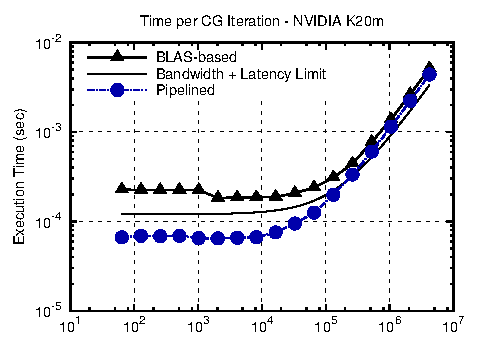
\includegraphics[width=0.85\textwidth]{figures/cg-k20m-3}
 \end{center}

 \begin{itemize}
  \item   \vspace*{-0.3cm} {\small (2D Finite Difference Discretization)}
 \end{itemize}
 \end{block}   
\end{frame}



\begin{frame}[fragile]{Performance Modeling: Conjugate Gradients}
 \begin{block}{Benefits of Pipelining also for Large Matrices}
 \begin{center}
  \vspace*{-0.2cm}
  \hspace*{-1.5cm}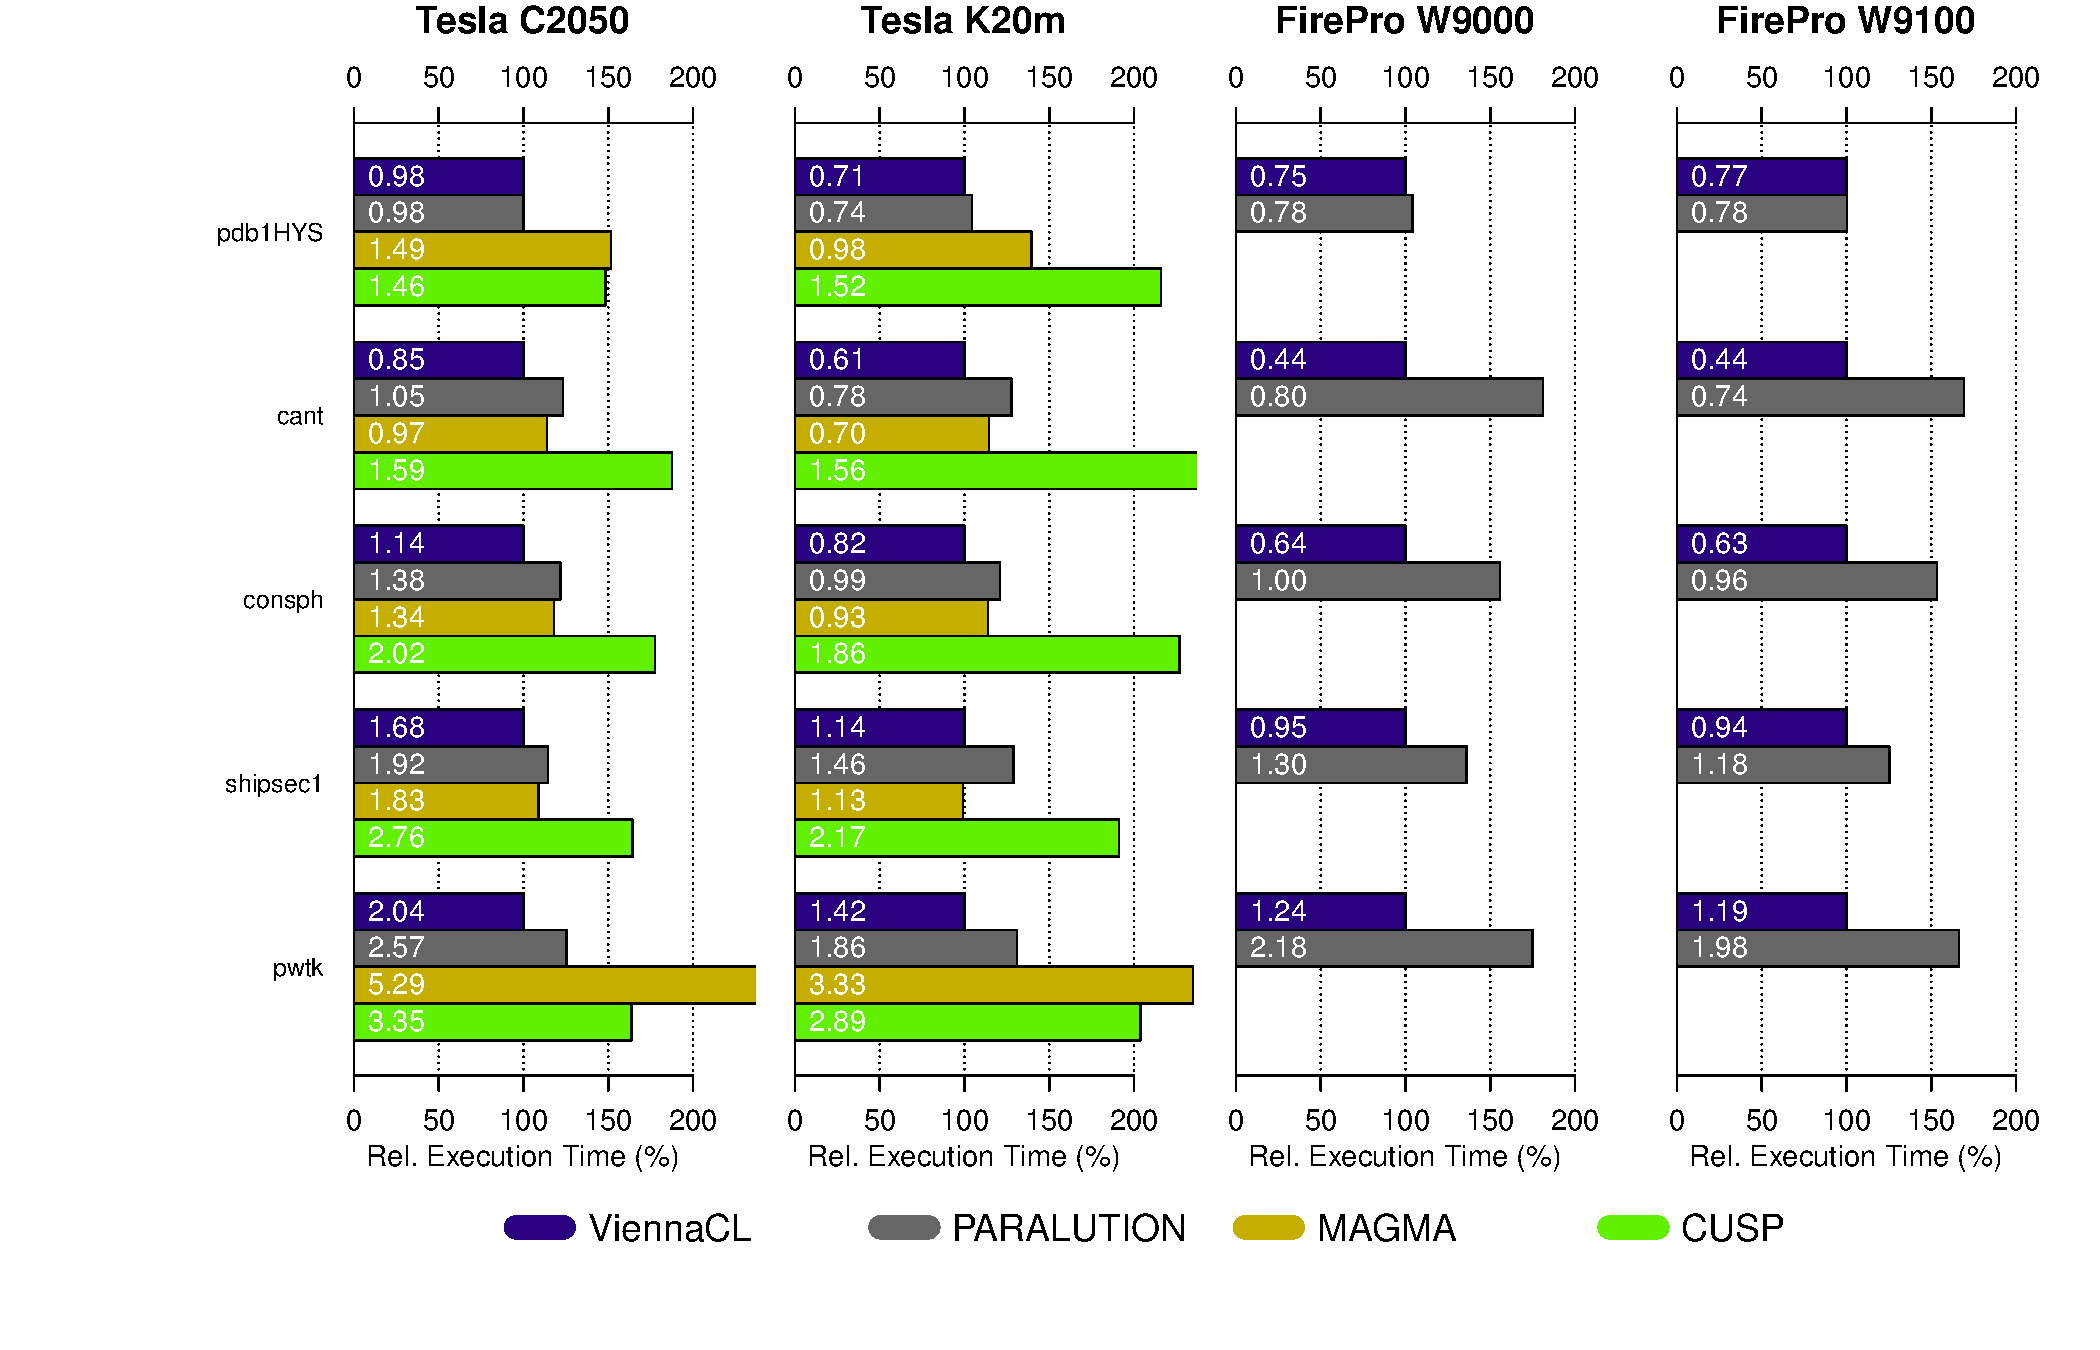
\includegraphics[width=1.05\textwidth]{figures/cg}
 \end{center}
  \vspace*{0.2cm}

 \end{block}   
\end{frame}




% Sparse Matrix transposition

\begin{frame}[fragile]{Performance Modeling: Sparse Matrix Transpose}
 \begin{block}{Sparse Matrix Transposition}
  \begin{itemize}
   \item Compute $B = A^{\mathrm{T}}$
   \item $A$ and $B$ using sparse storage schemes
  \end{itemize}
 \end{block}   
 
  \begin{block}{Row-Wise Datastructures}
  \begin{itemize}
   \item \lstinline|std::vector<std::map<int, double> >|
   \item \lstinline|std::vector<boost::flat_map<int, double> >|
   \item Compressed Sparse Row
  \end{itemize}
 \end{block}   

\end{frame}



\begin{frame}[fragile]{Performance Modeling: Sparse Matrix Transpose}

 \begin{block}{Simplest Case: STL}
  \begin{lstlisting}
for (int i=0; i<N; ++i)
  for (auto col = A[i].begin(); col != A[i].end(); ++col)
    B[col->index][i] = col->value
  \end{lstlisting}
 \end{block}   
 
 %\pause
  \begin{block}{More Work: CSR}
  \begin{itemize}
   \item Compute number of nonzeros per row in $B$
   \item Allocate data arrays for $B$
   \item Exclusive scan to find entry points per row
   \item Populate $B$
  \end{itemize}
 \end{block}   

 %\pause
   \begin{block}{Performance Modeling}
  \begin{itemize}
   \item Read and write each nonzero entry at least once
   \item Low arithmetic intensity: Bandwidth limited!
   \item $T(N) = 2 \times (4+8) \times \mathrm{nnz}(N) / \mathrm{Bandwidth}$
  \end{itemize}
 \end{block}   

\end{frame}


\begin{frame}[fragile]{Performance Modeling: Sparse Matrix Transpose}

 \begin{center}
%   \only<1>{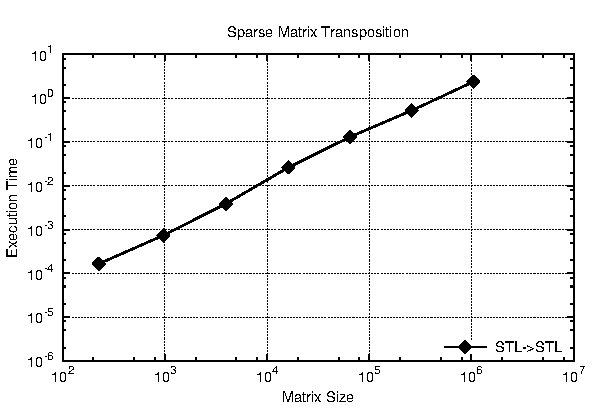
\includegraphics[width=0.99\textwidth]{figures/transpose-1}}
%   
%   \only<2>{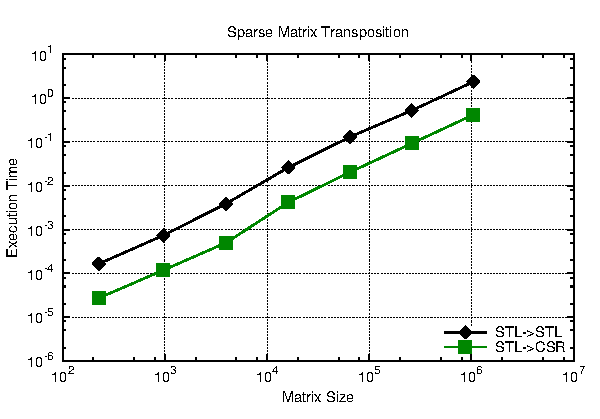
\includegraphics[width=0.99\textwidth]{figures/transpose-2}}
%   
%   \only<3>{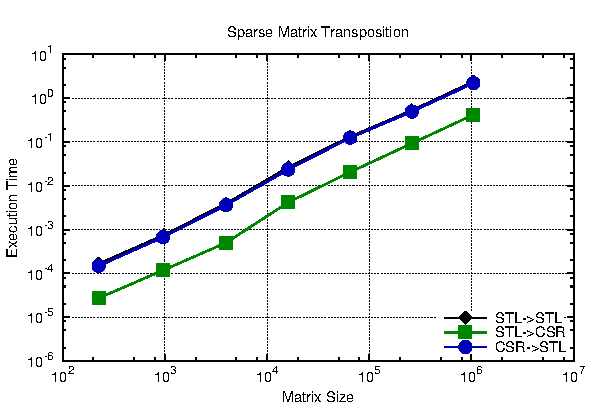
\includegraphics[width=0.99\textwidth]{figures/transpose-3}}
%   
%   \only<4>{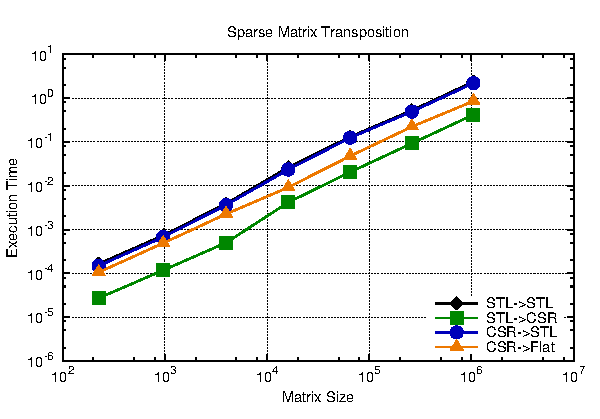
\includegraphics[width=0.99\textwidth]{figures/transpose-4}}
%   
%   \only<5>{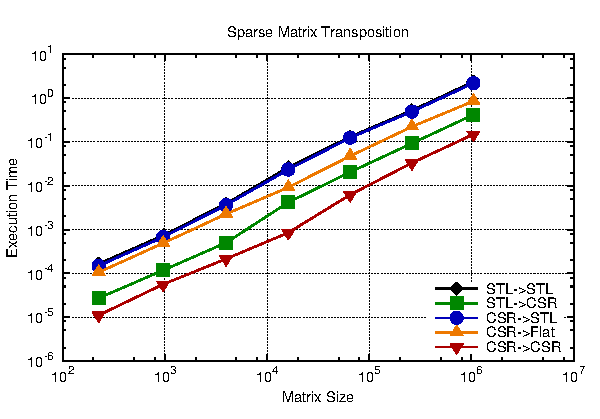
\includegraphics[width=0.99\textwidth]{figures/transpose-5}}
  
  \only<1>{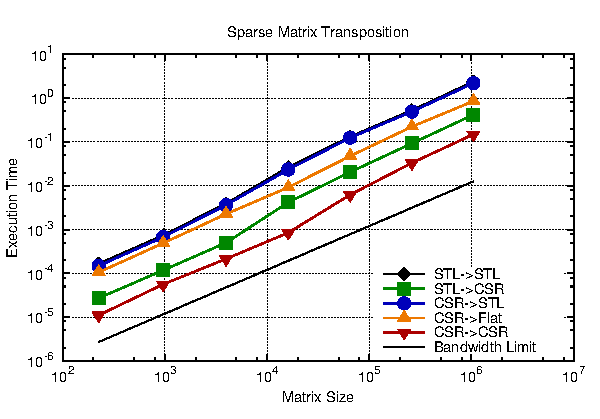
\includegraphics[width=0.99\textwidth]{figures/transpose-6}}
 \end{center}


\end{frame}


% Sparse Matrix-Matrix multiplication?

